\documentclass{article}
% For math environments
\usepackage{amsmath, amsfonts}
% For links
\usepackage[colorlinks=true,
    linkcolor = blue,
    urlcolor  = blue,
    citecolor = blue,
    anchorcolor = blue]{hyperref}
% Put space between paragraphs
\usepackage{parskip}
% For figures
\usepackage{tikz}
% Set the margins to not be ridiculous
\usepackage[margin=0.75in]{geometry}
% For multiple columns
\usepackage{multicol}
% For controlling enum/itemize spacing and indentation
\usepackage{enumitem}
% More math symbols
\usepackage{amssymb}
% To change enumerate labels

% For tikz plots
\usepackage{pgfplots}
% This isn't needed but avoids a compiler warning
\pgfplotsset{compat=1.16}

% Allow multi-line equations to be broken across pages
\allowdisplaybreaks

% Use @ as a letter
\makeatletter

% Scale down all tikz coordinates while maintaining font size
\tikzset{every picture/.style={scale=0.45, every picture/.style={}}}


% Macros
% Monospace code
\def\code#1{\texttt{#1}}

% Greek letters
\def\a{\alpha}
\def\b{\beta}
\def\g{\gamma}
\def\d{\delta}
\def\D{\Delta}

% Commands that make life easier
\newcommand\gath[1]{\begin{gather} #1 \end{gather}}
\newcommand\ali[1]{\begin{align} #1 \end{align}}
\newcommand\parens[1]{\left( #1 \right)}
\newcommand\squares[1]{\left[ #1 \right]}
\newcommand\braces[1]{\left\{ #1 \right\}}
\newcommand\angles[1]{\left\langle #1 \right\rangle}
\newcommand\deriv[2]{\frac{d #1}{d #2}}
\newcommand\abs[1]{\left| #1 \right|}
\newcommand\floor[1]{\left\lfloor #1 \right\rfloor}
\DeclareMathOperator{\lcm}{lcm}
\def\non{\nonumber \\}

% Multiline equation space
\def\mlesp{\hspace{1.2cm}}

% For grid diagrams
\newcommand\gridbox[3]{\draw (#1,#2) rectangle (#1+1,#2+1) node[pos=.5] {#3};}
\newcommand\gridboxh[3]{\draw[fill=red!20] (#1,#2) rectangle (#1+1,#2+1) node[pos=.5] {#3};}
\newcommand\gridboxb[3]{\draw[fill=black] (#1,#2) rectangle (#1+1,#2+1) node[pos=.5] {#3};}
\newcommand\gridsym[3]{\node at (#1+0.5,#2+0.5) {$#3$};}
\newcommand\gridblank[2]{\filldraw[draw=gray, color=gray] (#1,#2) rectangle (#1+1,#2+1);}
\newcommand\gridcirc[2]{\draw (#1 + 0.5,#2 + 0.5) circle (0.25);}
\newcommand\cwlab[3]{
  \def\dd{0.15}
  \draw (#1 + \dd - 0.03, #2 + 1 - \dd) node {\scriptsize #3};
}

\def\bbw{3.5}
\def\bbh{2}
\newcommand\bigbox[3]{\draw (#1*\bbw,#2*\bbh) rectangle (#1*\bbw+\bbw,#2*\bbh+\bbh) node[pos=.5] {#3};}
\newcommand\bbtextr[3]{\node[right] at (#1*\bbw,#2*\bbh+0.5*\bbh) {#3};}
\newcommand\bbtextb[3]{\node[align=center] at (#1*\bbw+0.5*\bbw,#2*\bbh+0.5*\bbh) {#3};}

% Box puzzle stock answer
\newcommand\boxans[1]{
  Logic was used to deduce the solution:

  #1

  This was verified using Python as well as shown to be unique with a brute force approach.
}

% Multiple numbers
\newcommand\mn[1]{$#1$'s}

% Commands for problems
\newcommand\problem[4]{
  \section*{#1}

  Question: #3
  
  Answer: #2
  
  Explanation: #4
}
\newcommand\aproblem[4]{\problem{Dec #1}{#2}{#3}{#4}}
\newcommand\cproblem[4]{\problem{Problem #1}{#2}{#3}{#4}}

\def\advent@xxiv@i{
  Eve writes down five different positive integers.
  The sum of her integers is $16$. What is the product of her integers?
}

\def\advent@xxiv@ii{
  $14$ is the smallest even number that cannot be obtained by rolling two $6$-sided dice and finding the product of the numbers rolled.

  What is the smallest even number that cannot be obtained by rolling one hundred $100$-sided dice and finding the product of the numbers rolled?
}

\def\advent@xxiv@iii{
  There are $5$ ways to write $5$ as the sum of positive odd numbers:
  \begin{itemize}
    \item $1 + 1 + 1 + 1 + 1$
    \item $1 + 1 + 3$
    \item $3 + 1 + 1$
    \item $1 + 3 + 1$
    \item $5$
  \end{itemize}

  How many ways are there to write $14$ as the sum of positive odd numbers?
}

\def\advent@xxiv@iv{
  The geometric mean of a set of $n$ numbers is computed by mulitplying all the numbers together, then taking the $n$th root.
  The factors of $9$ are $1$, $3$, and $9$.
  The geometric mean of these factors is
  \gath{
    \sqrt[3]{1 \times 3 \times 9} = \sqrt[3]{27} = 3
  }
  What is the smallest number where the geometric mean of its factors is $13$?
}

\def\advent@xxiv@v{
  The sum of $11$ consecutive integers is $2024$.
  What is the smallest of the $11$ integers?
}

\def\advent@xxiv@vi{Put the digits 1 to 9 (using each digit exactly once) in the boxes so that the sums are correct. The sums should be read left to right and top to bottom ignoring the usual order of operations. For example, 4+3×2 is 14, not 10. Today's number is the product of the numbers in the red boxes.
  The number $n$ has $55$ digits.
  All of its digits are $9$.
  What is the sum of the digits of $n^3$?
}

\def\advent@xxiv@vii{
  What is the obtuse angle in degrees between the minute and hour hands of a clock at 08:22?
}

\def\advent@xxiv@viii{
  It is possible to arrange $4$ points on a plane and draw non-intersecting lines between them to form $3$ non-overlapping triangles:

  \begin{center}
    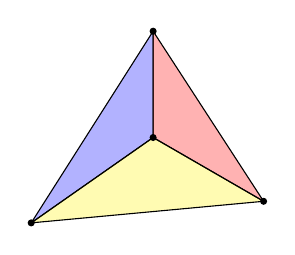
\begin{tikzpicture}
      \def\ds{3}
      \def\pa{(0: 0)}
      \def\pb{(90: \ds)}
      \def\pc{(215: 1.4*\ds)}
      \def\pd{(-30: 1.2*\ds)}

      \def\bcr{3}
      \def\scr{0.55*\bcr}
      \def\sca{34}
      \def\mcr{0.7*\bcr}
      \def\mca{142}
      \def\pr{0.1}

      % Triangles
      \draw[fill=blue,fill opacity=0.3] \pa -- \pb -- \pc -- cycle;
      \draw[fill=red,fill opacity=0.3] \pa -- \pb -- \pd -- cycle;
      \draw[fill=yellow,fill opacity=0.3] \pa -- \pd -- \pc -- cycle;

      % Points
      \fill \pa circle (\pr);
      \fill \pb circle (\pr);
      \fill \pc circle (\pr);
      \fill \pd circle (\pr);
    \end{tikzpicture}
  \end{center}

  It is not possible to make more than $3$ triangles with $4$ points.

  What is the maximum number of non-overlapping triangles that can be made by arranging $290$ points on a plane and drawing non-intersecting lines between them?
}

\def\advent@xxiv@ix{
  Put the digits $1$ to $9$ (using each digit exactly once) in the boxes so that the sums are correct.
  The sums should be read left to right and top to bottom ignoring the usual order of operations.
  For example, $4 + 3 \times 2$ is $14$, not $10$.
  Today's number is the product of the numbers in the red boxes.

  \grid@advent@xxiv@ix{}{}{}{}{}{}{}{}{}
}

\def\advent@xxiv@x{
  A number is a palindrome if it's the same when its digits are written in reverse order.

  What is the sum of all the numbers between $10$ and $100$ that are palindromes?
}

\def\advent@xxiv@xi{
  There are $6$ sets of integers between $1$ and $5$ (inclusive) that contain an odd number of numbers whose median value is $3$:

  \begin{itemize}
    \item $\braces{3}$
    \item $\braces{1,3,4}$
    \item $\braces{2,3,4}$
    \item $\braces{1,3,5}$
    \item $\braces{2,3,5}$
    \item $\braces{1,2,3,4,5}$
  \end{itemize}

  How many sets of integers between $1$ and $11$ (inclusive) are there that contain an odd number of numbers whose median value is $5$?
}

\def\advent@xxiv@xii{
  Holly picks a three-digit number.
  She then makes a two-digit number by removing one of the digits.
  The sum of her two numbers is $309$.
  What was Holly's original three-digit number?
}

\def\advent@xxiv@xiii{
  Today's number is given in this crossnumber.
  No number in the completed grid starts with $0$.

  \begin{multicols}{2}
    \crossnumstd{}{}{}{}{}{}{}{}{}

    \vfill\null
    \columnbreak

    \begin{center}
      \textbf{Across}

      \begin{tabular}{clc}
        \textbf{1} & Today's number.  & (\textbf{3}) \\
        \textbf{4} & Two times 5A.    & (\textbf{3}) \\
        \textbf{5} & A multiple of 1. & (\textbf{3})
      \end{tabular}

      \textbf{Down}

      \begin{tabular}{clc}
        \textbf{1} & Sum of digits is 15. & (\textbf{3}) \\
        \textbf{2} & Sum of digits is 19. & (\textbf{3}) \\
        \textbf{3} & Three times 5A.      & (\textbf{3})
      \end{tabular}
    \end{center}
  \end{multicols}
}

\def\advent@xxiv@xiv{
  $15^3$ is $3375$.
  The last $3$ digits of $15^3$ are $375$.

  What are the last $3$ digits of $15^{1234567890}$?
}

\def\advent@xxiv@xv{
  The number $2268$ is equal to the product of a square number (whose last digit is not $0$) and the same square number with its digits reversed: $36 \times 63$.

  What is the smallest three-digit number that is equal to the product of a square number (whose last digit is not $0$) and the same square number with its digits reversed?
}

\def\advent@xxiv@xvi{
  Put the digits $1$ to $9$ (using each digit exactly once) in the boxes so that the sums are correct.
  The sums should be read left to right and top to bottom ignoring the usual order of operations.
  For example, $4 + 3 \times 2$ is $14$, not $10$.
  Today's number is the product of the numbers in the red boxes.

  \grid@advent@xxiv@xvi{}{}{}{}{}{}{}{}{}
}

\def\advent@xxiv@xvii{
  The number $40$ has $8$ factors: $1$, $2$, $4$, $5$, $8$, $10$, $20$, and $40$.

  How many factors does the number $2^{26} \times 5 \times 7^5 \times 11^2$ have?
}

\def\advent@xxiv@xviii{
  TODO
}

\def\card@xxiv@i{
  What is the largest number you can make by using the digits $1$ to $4$ to make two $2$-digit numbers, then mutiplying the two numbers together?
}

\def\card@xxiv@ii{
  What is the largest number you can make by using the digits $0$ to $9$ to make a $2$-digit number and an $8$-digit number, then mutiplying the two numbers together?
}

\def\card@xxiv@iii{
  The expansion of $(2x+3)^2$ is $4x^2 + 12x + 9$.
  The sum of the coefficients of $4x^2 + 12x + 9$ is $25$.
  What is the sum of the coefficients of the expansion of $(30x + 5)^2$?
}

\def\card@xxiv@iv{
  What is the sum of the coefficients of the expansion of $(2x+1)^{11}$?
}

\def\card@xxiv@v{
  What is the geometric mean of all the factors of $41306329$?
}

\def\card@xxiv@vi{
  What is the largest number for which the geometric mean of all its factors is $92$?
}

\def\card@xxiv@vii{
  What is the sum of all the factors of $7^4$?
}

\def\card@xxiv@viii{
  How many numbers between $1$ and $28988500000$ have an odd number of factors?
}

\def\card@xxiv@ix{
  Eve found the total of the $365$ consecutive integers starting at $500$ and the total of the next $365$ consecutive integers, then subtracted the smaller total from the larger total.
  What was her result?
}

\def\card@xxiv@x{
  Eve found the total of the $n$ consecutive integers starting at a number and the total of the next $n$ consecutive integers, then subtracted the smaller total from the larger total.
  Her result was $22344529$.
  What is the largest possible value of $n$ that she could have used?
}


\begin{document}

\title{MS Scroggs 2022 Christmas Card Solutions}
\author{Dan Whitman}
\date{}

\maketitle

Link to the online card: \href{https://www.mscroggs.co.uk/blog/98}{https://www.mscroggs.co.uk/blog/98}

\cproblem{1}{5}{\card@xxii@i}{
  Just working through the primes starting at $1$, the answer is clearly $5$, which is two more than $3$ and two less than $7$, both of which are also prime.
}

\newcommand\sumo[1]{s_\mathrm{o}\parens{#1}}
\cproblem{2}{49}{\card@xxii@ii}{
  While this would be really simple to just manually calculate, it is more fun (though perhaps more work) to derive an easier formula.
  Clearly the sum of the first $n$ odd numbers is going to be
  \gath{
    \sumo{n} = \sum_{k=1}^n (2k - 1) = 2 \sum_{k=1}^n k - \sum_{k=1}^n 1 = \frac{2n(n+1)}{2} - n = n^2 \,.
  }
  Thus our answer is $\sumo{7} = 7^2 = 49$.
}

\cproblem{3}{33}{\card@xxii@iii}{
  From the equation derived in the previous problem, clearly the answer is $\sqrt{1089} = 33$.
}

\cproblem{4}{1}{\card@xxii@iv}{
  Since $7$ is prime, the quotient group $\ints/7\ints$ is cyclic, and indeed $4$ is a generator for it.
  From this it follows that \emph{any} integer can be obtained by adding only integer multiples of $4$ and $7$.
  As an example, clearly $2 \cdot 4 - 1 \cdot 7 = 1$, which is of course the smallest positive integer period.
}

\cproblem{5}{80}{\card@xxii@v}{
  This is similar to the previous problem, but not so straightforward because our two integers are not coprime.
  In particular, $\gcd(240, 400) = 80$ so that only integer multiples of $80$ are obtainable by adding integer multiples of $240$ and $400$.
  Hence, our answer is of course $80$, noting that $2 \cdot 240 - 1 \cdot 400 = 80$ as an example of how to attain this.
}

\cproblem{6}{20}{\card@xxii@vi}{
  Here we can leverage the solution of the 2022, Dec~6 problem.
  There, it was reasoned that, for a digital sum of $1 \leq s \leq 9$, the number of $m$-digit numbers with this digital sum and for which there are no nonzero digits is the recursive function
  \gath{
    N_m(s) = \begin{cases}
      1                             & m = 1         \\
      \sum_{j=m-1}^{s-1} N_{m-1}(j) & 1 < m \leq 9.
    \end{cases} \label{eqn:06:rec}
  }
  It was also derived that, in particular,
  \gath{
    N_3(s) = \frac{(s-1)(s-2)}{2}.
  }
  Hence, for $4$-digit numbers we have
  \ali{
    N_4(s) &= \sum_{j=3}^{s-1} N_3(j) = \sum_{j=3}^{s-1} \frac{(j-1)(j-2)}{2} = \frac{1}{2} \sum_{j=3}^{s-1} \parens{j^2 - 3j + 2} = \frac{1}{2} \parens{\sum_{j=3}^{s-1} j^2 - 3 \sum_{j=3}^{s-1} j + 2 \sum_{j=3}^{s-1} 1} \non
    &= \frac{1}{2}\squares{\frac{s(s-1)(2s-1)}{6} - (2^2 + 1^2) - \frac{3s(s-1)}{2} + 3(2 + 1) + 2(s-3)} \non
    &= \frac{1}{2}\squares{\frac{2s^3 - 12s^2 + 22s - 12}{6}} = \frac{s^3 - 6s^2 + 11s - 6}{6}.
  }
  So our answer is then $N_4(7) = 20$, which was also verified with a brute force search Python program.
}

\cproblem{7}{64}{\card@xxii@vii}{
  This is just like the previous problem except that we are looking at all positive integers instead of just the $4$-digit integers.
  Again, we can use the results of the 2022, Dec~6 problem, according to which this number for the general digital sum $s$ is
  \gath{
    N_s = \sum_{m=1}^s N_m(s). \label{eqn:07:Ns}
  }
  Just like the Dec~6 problem, we shall not undergo the tedium of computing $N_5(s)$, $N_6(s)$, or $N_7(s)$, but instead implement \eqref{eqn:07:Ns} along with the recursive function \eqref{eqn:06:rec} in Python to arrive at our answer $N_7 = 64$.
  As before, this result was also verified with a brute force search in the Python program.
}

\cproblem{8}{2836}{\card@xxii@viii}{
  Suppose that the original $4$-digit number is $d_3 d_2 d_1 d_0$ where of course $0 \leq d_i \leq 9$ for all $0 \leq i \leq 3$.
  Now, it \emph{has} to be that the least significant digit is the one that was removed since otherwise the sum would end in $d_0 + d_0 = 2d_0$ so that it would have to end in an even digit.
  Since the sum 
  ends in a $9$ though, it must be that the $3$-digit number is $d_3 d_2 d_1$, and our sum is
  \begin{center}
    \begin{tabular}{ccccc}
          & $d_3$ & $d_2$ & $d_1$ & $d_0$ \\ 
      $+$ &       & $d_3$ & $d_2$ & $d_1$ \\
      \hline
          & 3 & 1 & 1 & 9
    \end{tabular}
  \end{center}
  Clearly either $d_3 = 3$ and nothing is carried from the $d_2 + d_3$ digit, or else $d_3 = 2$ and a $1$ \emph{is} carried.
  It must be the latter case since, in the former case, clearly $d_2 + d_3 = d_2 + 3 > 1$ so that this would have to be an $11$ instead and thus would carry, which contradicts that case.
  So, since $d_3 = 2$ and the previous digit's sum must be $11$, we have a similar situation in that either $d_2 = 9$ and there is no carry from the $d_1 + d_2$ digit, or else $d_2 = 8$ and there is a carry.
  For the same reason as before it must be that there \emph{is} a carry so that $d_2 = 8$.

  Now, there can be no carry from the least significant $d_0 + d_1$ digit because there is no way for this sum to reach $19$.
  Thus, we have that $d_1 + d_2 = d_1 + 8 = 11$ so that clearly $d_1 = 3$.
  Then of course $d_0 + d_1 = d_0 + 3 = 9$, and hence $d_0 = 6$.
  Therefore, the original number is $d_3 d_2 d_1 d_0 = 2836$, and indeed it is trivial to verify that $2836 + 283 = 3119$ as required.
}

\cproblem{9}{TODO}{\card@xxii@ix}{
  TODO
}

\cproblem{10}{TODO}{\card@xxii@x}{
  TODO
}

\cproblem{11}{TODO}{\card@xxii@xi}{
  TODO
}

\end{document}
